% EE 604 course project write-up.
% Based on the CVPR 2026 Paper Template; see https://github.com/cvpr-org/author-kit
% (same template as https://www.overleaf.com/latex/templates/cvpr-2022-author-kit/qbmjsdxryffn)

\documentclass[10pt,twocolumn,letterpaper]{article}

%%%%%%%%% PAPER TYPE
\usepackage[pagenumbers]{cvpr} % final version with names and page numbers (no review line numbers)

% Import additional packages in the preamble file, before hyperref
%% This file contains a number of tweaks that are typically applied to the main document.
%% They are not enabled by default, but can be enabled by uncommenting the relevant lines.

%%
%% Inline annotations; for predefined colors, refer to "dvipsnames" in the xcolor package:
%% https://tinyurl.com/overleaf-colors
%%
\newcommand{\red}[1]{{\color{red}#1}}
\newcommand{\todo}[1]{{\color{red}#1}}
\newcommand{\TODO}[1]{\textbf{\color{red}[TODO: #1]}}
%%
%% disable for camera ready / submission by uncommenting these lines  
%%
% \renewcommand{\TODO}[1]{}
% \renewcommand{\todo}[1]{#1}

%%
%% work harder in optimizing text layout. Typically shrinks text by 1/6 of page, enable
%% it at the very end of the writing process, when you are just above the page limit
%%
% \usepackage{microtype}

%%
%% fine-tune paragraph spacing
%%
% \renewcommand{\paragraph}[1]{\vspace{.5em}\noindent\textbf{#1.}}

%%
%% globally adjusts space between figure and caption
%%
% \setlength{\abovecaptionskip}{.5em}


%%
%% Allows "the use of \paper to refer to the project name"
%% with automatic management of space at the end of the word
%%
% \usepackage{xspace}
% \newcommand{\paper}{ProjectName\xspace}

%%
%% Commonly used math definitions
%%
% \DeclareMathOperator*{\argmin}{arg\,min}
% \DeclareMathOperator*{\argmax}{arg\,max}

%%
%% Tigthen underline
%%
% \usepackage{soul}
% \setuldepth{foobar}
%%
%% EE 604 project additions
%%
\usepackage{listings}
\usepackage{multirow}
\usepackage{eurosym}
\newcommand{\gest}[1]{\texttt{#1}}
\lstset{basicstyle=\ttfamily\scriptsize, breaklines=true, columns=fullflexible,
        keepspaces=true, showstringspaces=false, frame=single, framerule=0.3pt,
        numbers=left, numberstyle=\tiny\color{gray}, language=Python,
        commentstyle=\color{OliveGreen}, keywordstyle=\color{NavyBlue},
        stringstyle=\color{BrickRed}}


\definecolor{cvprblue}{rgb}{0.21,0.49,0.74}
\usepackage[pagebackref,breaklinks,colorlinks,allcolors=cvprblue]{hyperref}

%%%%%%%%% PAPER ID
\def\paperID{EE604}
\def\confName{EE 604}
\def\confYear{2026}

% Title, authors (from team.json) and a few values generated by make_report.py
\newcommand{\GitHubURL}{https://github.com/gunasekharkaranam/gesture-mouse-keyboard}
\newcommand{\Hardware}{an ordinary laptop CPU without a GPU}
\newcommand{\Camera}{EDIT: e.g. built-in 720p laptop webcam}
\newcommand{\DatasetSentence}{Because no public dataset matches our gesture set and our control setting, we recorded our own: 15378 labelled frames from 3 users (between 1880 and 2530 per gesture) and 0 hand-crop images.}
\newcommand{\DatasetShort}{15378 keypoint samples and 0 hand crops from 3 users}
\newcommand{\AccMLP}{99.74}
\newcommand{\AccRules}{89.89}
\newcommand{\LosoMLP}{96.64}
\newcommand{\LosoRules}{89.83}
\newcommand{\PersZero}{97.35}
\newcommand{\PersK}{98.01}
\newcommand{\ObsClassification}{Our MLP with the full feature set reaches 99.74\% accuracy (macro-F1 99.74\%) in 0.72\,ms per sample, compared with 89.89\% for the rule-based method. The feature design matters: the same MLP on raw coordinates reaches 99.67\%, so normalisation and shape features change accuracy by +0.07 points. Augmentation changes accuracy by -0.03 points on this split. Random Forest is slightly more accurate (99.84\%), but takes 10.87\,ms per sample, 15.1$\times$ the MLP's time. \Cref{fig:cm} shows the remaining confusions.}
\newcommand{\ObsLoso}{Averaged over 3 held-out users, our MLP reaches 96.64\%, against 89.83\% for the rules, 90.19\% for the SVM and 93.88\% for an MLP on raw coordinates without augmentation. The hardest user is bhuvana (94.39\%), which motivates personalization (\cref{fig:personal}).}
\newcommand{\ObsCNN}{The keypoint MLP is 0.20 points lower in accuracy than the CNN (99.74\% vs.\ 99.94\%), while being 6$\times$ faster and 12$\times$ smaller. Working on keypoints also removes the influence of background and lighting, which the CNN has to learn from data.}
\newcommand{\ObsPers}{Averaged over 3 users, accuracy on a new user is 97.35\% without calibration and rises to 98.01\% with $K=20$ samples per gesture (about one second of recording per gesture).}
\newcommand{\ObsFilter}{Compared with the raw cursor, the One-Euro filter reduces jitter by 38.5\% (from 4.21 to 2.59 px/frame) with 11\,ms of lag. The moving average gives 3.57 px/frame jitter but 64\,ms lag, and the Kalman filter 3.66 px/frame with 32\,ms lag. The One-Euro filter is the best trade-off because its cutoff rises with hand speed.}
\newcommand{\ObsVoting}{Voting ($N{=}5,k{=}3$) lowers the number of gesture changes from 70.0 to 21.2 per minute and the short (1--2 frame) false segments from 31.0 to 0.3 per minute, and detects 30 clicks (without voting: 50) for the 30 the user made.}
\newcommand{\ObsAnchor}{With the fingertip as anchor, the cursor moves 182.5\,px on average while the click is being made; with the knuckle it moves only 53.4\,px (71\% less), so small targets are not missed.}
\newcommand{\ObsSystem}{The complete pipeline runs at 32.2 FPS with 11.5\,ms of processing per frame (95th percentile 14.8\,ms), i.e.\ in real time on a CPU.}
\newcommand{\ObsClick}{\todo{Result not available yet: run \texttt{python experiments/click\_test.py --method gesture --user NAME}.}}
\newcommand{\ObsTyping}{\todo{Result not available yet: run \texttt{python experiments/typing\_test.py --user NAME}.}}
\newcommand{\ObsAbstract}{In experiments with 3 users, the system reaches 96.6\% gesture accuracy on users not seen in training (rule-based: 89.8\%), removes 38\% of the cursor jitter, cuts gesture flicker by 70\%, reduces cursor drift during a click by 71\% and runs at 32 FPS on a laptop CPU.}
\newcommand{\ObsConclusion}{In experiments with 3 users, the system reaches 96.6\% gesture accuracy on users not seen in training (rule-based: 89.8\%), removes 38\% of the cursor jitter, cuts gesture flicker by 70\%, reduces cursor drift during a click by 71\% and runs at 32 FPS on a laptop CPU. Each proposed component gives a measurable improvement over the usual design, and together they make a webcam a practical touch-free mouse and keyboard.}

\title{Gesture Mouse and Air Keyboard: Robust Real-Time Computer Control with a Webcam using Invariant Hand-Keypoint Learning}
\author{Guna Sekhar Subbarao Karanam\\230537\\{\tt\small kgssekhar23@iitk.ac.in} \and VOOBA RAJKUMAR\\231173\\{\tt\small rajvk23@iitk.ac.in} \and GBHUVANA REDDY\\230408\\{\tt\small bhuvanar23@iitk.ac.in}\\[4pt] \small EE 604: Image Processing, IIT Kanpur, 2026}


\begin{document}
\maketitle
\begin{abstract}
Can a normal laptop webcam replace the mouse and the keyboard? We built a
system that watches the user's hand and turns hand gestures into real mouse
and keyboard actions: moving the cursor, left and right click, scrolling,
dragging and typing on an on-screen ``air keyboard''. It needs no gloves, no
special camera and no GPU. Simple versions of this idea already exist, but
they decide the gesture with fixed ``which fingers are up'' rules, so they fail
for new people and tilted hands, the cursor shakes, and it jumps away from the
target at the moment of a click. We fixed these problems one by one. We
first clean the 21 hand points found by MediaPipe so that position, size,
tilt and left/right hand no longer matter, and a small neural network then
learns the gestures from these cleaned points. A voting step over the last
five frames stops false clicks. The cursor follows the index-finger knuckle
instead of the fingertip, and a speed-aware One-Euro filter keeps it steady.
On a person the network had never seen, it recognised gestures with
\textbf{96.6\%} accuracy, against \textbf{89.8\%} for the usual rules. The
filter reduced cursor shake by \textbf{38\%} with only \textbf{11\,ms} of
delay. Voting turned 50 detected clicks into exactly 30 for 30 real pinches.
The knuckle cut the cursor jump during a click from 183\,px to 53\,px. The
whole system runs at \textbf{32 frames per second} on a laptop CPU.
\end{abstract}

\section{Introduction}
\label{sec:intro}

We touch a mouse and a keyboard all day. Sometimes touching them is a problem:
a doctor wearing gloves, a cook with dirty hands, a teacher standing far from
the laptop during a lecture, a shared screen in a public place, or a person
who finds small devices hard to hold. Almost every laptop already has a
webcam, so a mouse and keyboard that work with \emph{only the webcam} would
cost nothing and help all these people.

The idea is not new. Many open-source ``virtual mouse'' programs find the
hand with MediaPipe~\cite{zhang2020mediapipe}, check which fingers are up with
a few fixed rules, and move the cursor with the index fingertip. When we tried
this approach, it worked in a demo but was hard to use for real work. We saw
four problems:
\begin{enumerate}
\item \textbf{Rules break easily.} A slightly tilted hand, a hand far from the
camera, or simply a different person makes the fixed thresholds fail.
\item \textbf{The cursor shakes.} The detected hand points move a few pixels
in every frame even when the hand is still, so small buttons are hard to hit.
\item \textbf{The cursor jumps when you click.} To click, you pinch the thumb
and index finger. This moves the fingertip, and the cursor goes with it, just
when you need it to stay still.
\item \textbf{False clicks.} When the hand changes from one gesture to another,
the detector is wrong for a frame or two, and each wrong ``pinch'' frame
becomes a click.
\end{enumerate}

Our project is about solving these four problems, and about \emph{measuring}
that each fix really helps. We keep MediaPipe for finding the hand, and
everything after it is our own work:

\begin{itemize}
\item \textbf{A learned gesture classifier on cleaned hand points
(\cref{sec:features,sec:mlp}).} Before classification we remove the
effect of hand position, size, tilt and left/right hand. A small neural
network (an MLP with about 20\,k weights) then learns 7 gestures. We test it
on a person it has never seen.
\item \textbf{A stable cursor point (\cref{sec:cursor}).} The cursor follows the
index-finger \emph{knuckle}, which hardly moves during a pinch.
\item \textbf{A smart smoothing filter (\cref{sec:cursor}).} The One-Euro
filter~\cite{casiez2012oneeuro} smooths strongly when the hand is slow and
weakly when it is fast, so we get a steady cursor without delay.
\item \textbf{Voting over time (\cref{sec:voting}).} A gesture counts only
when it is seen in most of the last five frames with good confidence.
\item \textbf{Extras that make it usable (\cref{sec:actions}).} An air keyboard
with a ``hover-lock'' that types the right key, and a one-second
personalization for a new user.
\end{itemize}

The rest of the report follows the same story. \Cref{sec:related} looks at
what others have done. \Cref{sec:method} explains our method step by step,
and why we chose each step. \Cref{sec:exp} tests every step with our own
recorded data and live sessions. \Cref{sec:conclusion} sums up what we learned.

\section{Related Work}
\label{sec:related}

\paragraph{Recognising gestures from pixels.} Early systems found the hand
by its skin colour or by removing the background, and then described its shape;
Rautaray and Agrawal give a survey~\cite{rautaray2015survey}. These methods
break easily when the light or the background changes. Deep learning changed
the field. 3D CNNs with recurrent layers recognise moving gestures in
video~\cite{molchanov2016online}, and two-stage CNN systems detect and
classify gestures in real time~\cite{kopuklu2019realtime}. Large datasets
such as Jester~\cite{materzynska2019jester} and HaGRID~\cite{kapitanov2024hagrid}
made this possible. These models work very well, but they read raw pixels, so
they need a lot of training data and usually a GPU.

\paragraph{Finding hand points.} Another line of work finds the joints of
the hand instead of classifying pixels. Simon \etal~\cite{simon2017hand} detect
21 hand keypoints in a single image, and MediaPipe
Hands~\cite{zhang2020mediapipe} does this in real time on a phone CPU. Once we
have these 21 points, the background, skin colour and lighting are already
gone, and the gesture problem becomes much smaller: only 63 numbers per frame.
This is why we build on MediaPipe.

\paragraph{Virtual mouse programs.} Many open-source projects join MediaPipe
with PyAutoGUI~\cite{pyautogui}. They count fingers as ``up'' or ``down'' with
fixed thresholds and move the cursor with the fingertip. They are easy to
build, but, as said above, they are fragile, shaky and click by mistake.
They are also rarely measured: they show a demo, not numbers.

\paragraph{Smoothing and measuring a pointer.} Shaky input is usually
smoothed with a moving average or a Kalman filter~\cite{kalman1960}. Both
trade shake for delay. The One-Euro filter~\cite{casiez2012oneeuro} changes
its smoothing with the speed of the hand, which removes most of this
trade-off. Pointing devices are usually compared with Fitts'
law~\cite{fitts1954,soukoreff2004}.

\paragraph{Where our work fits.} We take the keypoint idea from the second
line of work and the virtual-mouse goal from the third, and we add what is
missing in between: a learned and position-free classifier tested on new
users, and a cursor that is designed and measured to be steady and reliable.

\section{Proposed Method}
\label{sec:method}

\begin{figure*}[t]
  \centering
  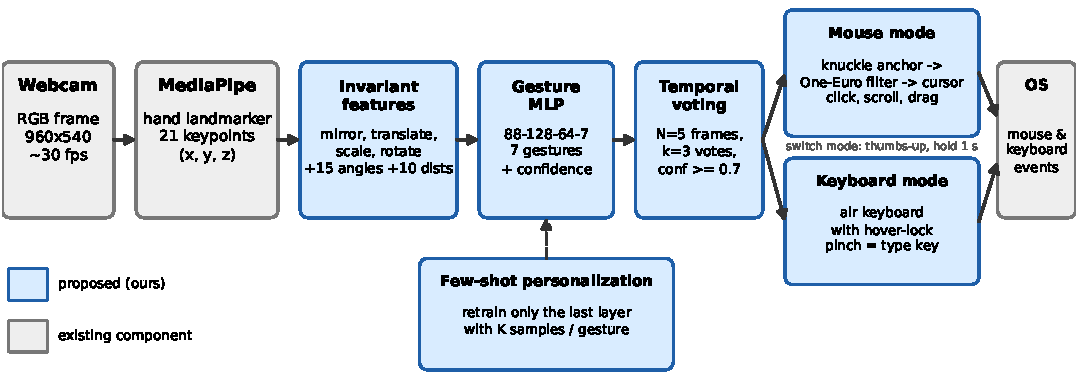
\includegraphics[width=\textwidth]{figures/overview.pdf}
  \caption{\textbf{Overview of our system.} Grey boxes are existing tools and
  blue boxes are our work. Each webcam frame gives 21 hand points. We clean
  them into 88 features, the Gesture MLP names the gesture, and voting makes
  the decision stable. The stable gesture then drives either the mouse
  (knuckle anchor and One-Euro filter) or the air keyboard (hover-lock). A new
  user can personalise the MLP with a few samples.}
  \label{fig:overview}
\end{figure*}

\Cref{fig:overview} shows the whole journey of one camera frame. In this
section we follow that frame from left to right. For each step we say what it
does and why we need it.

\subsection{Step 1: finding the hand}
The webcam gives a $960\times540$ colour frame about 30 times per second. We
flip it like a mirror, so that moving the hand to the right moves the cursor to
the right. MediaPipe's Hand Landmarker~\cite{zhang2020mediapipe} then returns
21 points $\mathbf{p}_i=(x_i,y_i,z_i)$ on the hand and tells us whether it is a
left or a right hand. Point 0 is the wrist, point 4 the thumb tip, point 5 the
index knuckle and point 8 the index tip. \emph{Why:} MediaPipe is accurate,
runs on a CPU and tracks the hand between frames, so most of our time budget
is left for the next steps.

\subsection{Step 2: cleaning the hand points}
\label{sec:features}
The same gesture can give very different raw numbers. The hand may be on the
left or the right of the image, near or far from the camera, tilted, or it may
be a left hand. A classifier would have to learn all these cases from data,
and our dataset is small. So we remove them by geometry
(\cref{fig:features}):
\begin{enumerate}
\item \textbf{Mirror} a left hand, $x_i \leftarrow 1-x_i$, so that one model
works for both hands.
\item \textbf{Move} the wrist to the origin: $\mathbf{q}_i=\mathbf{p}_i-\mathbf{p}_0$.
\item \textbf{Scale} by the palm size, the distance from the wrist to the
middle-finger knuckle: $\mathbf{q}_i \leftarrow \mathbf{q}_i/\lVert(\mathbf{p}_9-\mathbf{p}_0)_{xy}\rVert$.
\item \textbf{Rotate} the points so that the palm always points straight up.
\end{enumerate}
After this, a pointing hand looks the same wherever it is in the image. We
then add 15 bend angles (three joints per finger) and the 10 distances between
every pair of fingertips. These describe the hand shape directly: a pinch is
simply a small thumb-to-index distance. This gives $63+15+10=88$ numbers per
frame.

\begin{figure}[t]
  \centering
  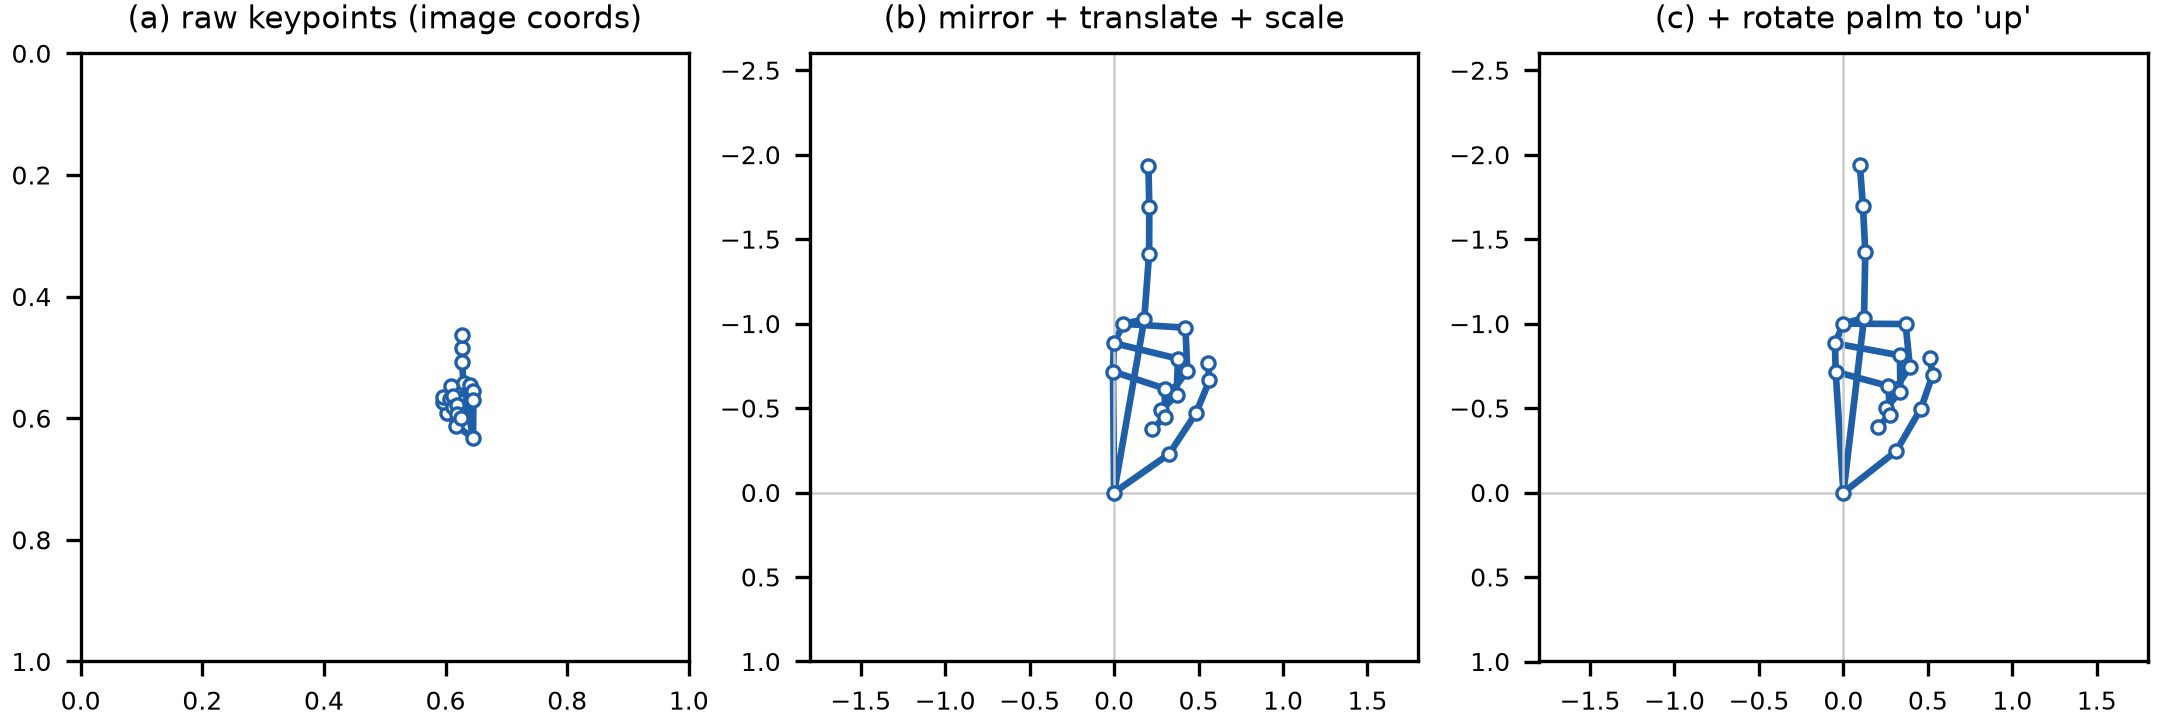
\includegraphics[width=\linewidth]{figures/features.png}
  \caption{\textbf{Cleaning the hand points} for one recorded frame: raw points
  in the image (a), after mirroring, moving and scaling (b), and after
  rotating the palm to point up (c).}
  \label{fig:features}
\end{figure}

\subsection{Step 3: naming the gesture with a neural network}
\label{sec:mlp}
We use 7 gestures (\cref{fig:gestures}). A small multi-layer perceptron (MLP)
reads the 88 features and outputs a probability for each gesture. Its layers
are $88\rightarrow128\rightarrow64\rightarrow7$, with batch
normalisation~\cite{ioffe2015batch}, ReLU and dropout~\cite{srivastava2014dropout}.
It has about 20\,k weights. To make it work for people who are not in the
training data, we show it four extra copies of every training frame. Each copy
is slightly rotated (up to $\pm20^\circ$), scaled (0.85 to 1.15), shifted and
given a little noise (data augmentation).

\emph{Why an MLP and not a CNN on the image?} After Step 2 the input is only 88
numbers, so a tiny network is enough. It runs in under a millisecond on a
CPU, and it never sees the background or the lighting. We check this choice
against an image CNN in \cref{sec:exp-cls}.

\begin{figure}[t]
  \centering
  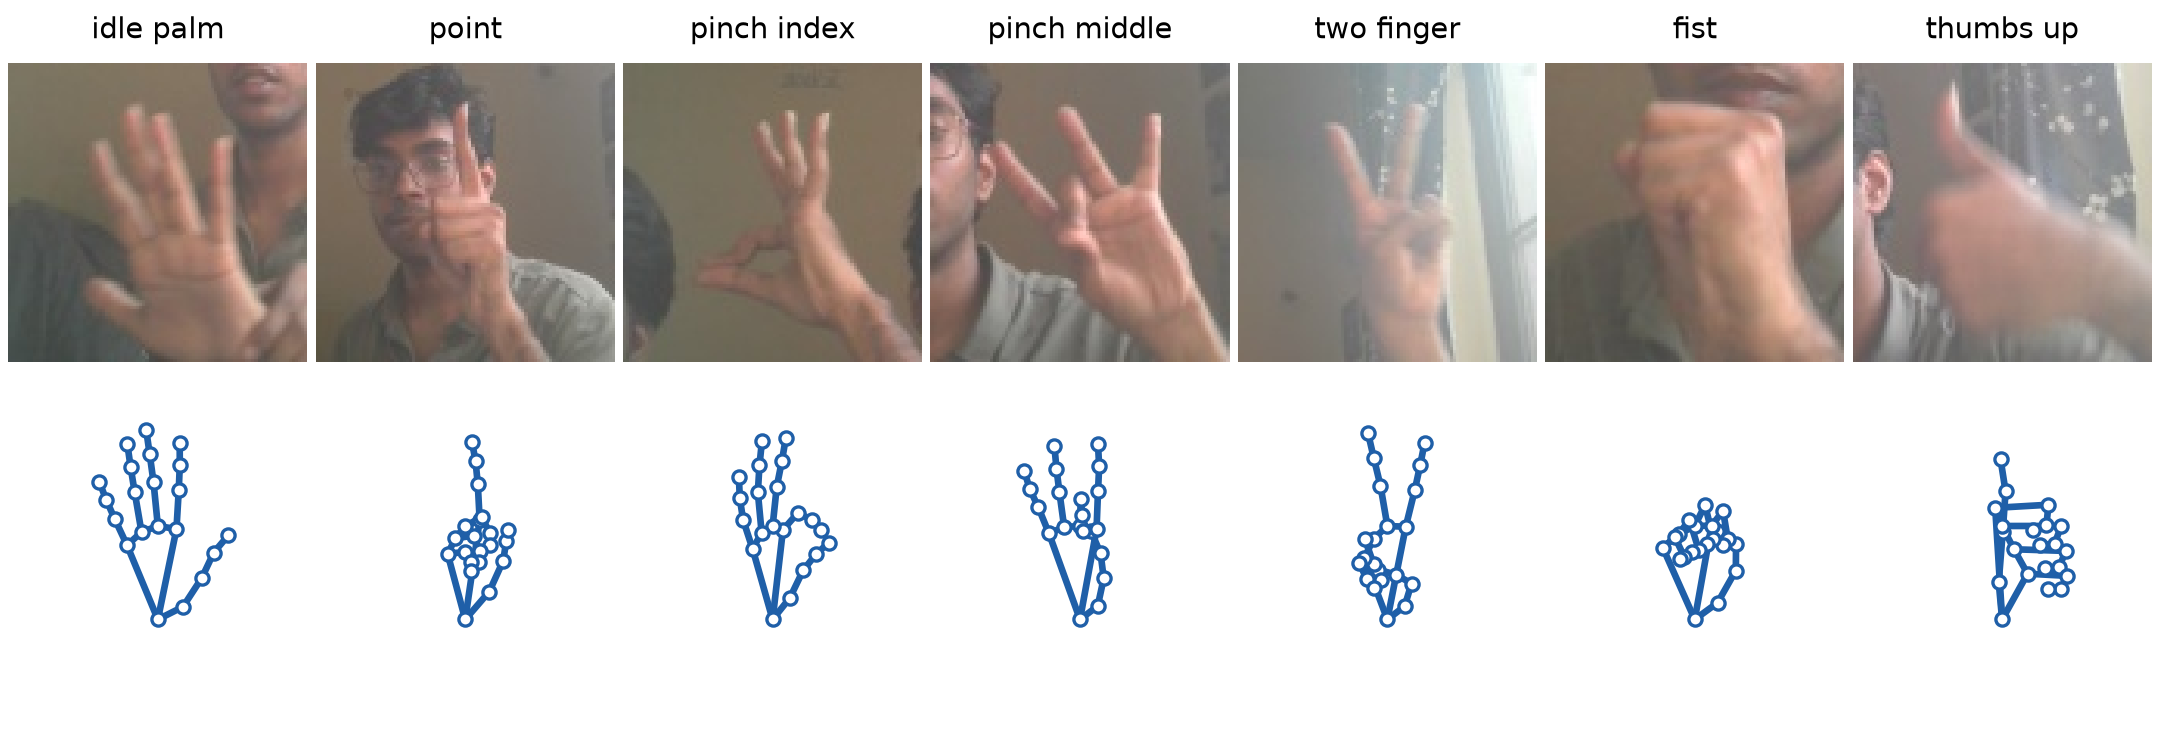
\includegraphics[width=\linewidth]{figures/gestures.png}
  \caption{\textbf{Our 7 gestures.} Top: a frame from our dataset. Bottom: the
  typical cleaned hand points of that gesture.}
  \label{fig:gestures}
\end{figure}

\subsection{Step 4: voting over time}
\label{sec:voting}
When the hand moves from ``point'' to ``pinch'', the network can be unsure for
a frame or two. If we acted on every frame, these short mistakes would become
clicks. So we keep the last $N=5$ predictions and their confidences, and we
change the \emph{stable} gesture only when one gesture gets at least $k=3$ of
the 5 votes \emph{and} its average confidence is at least 0.7. Otherwise the
old gesture stays. Actions happen only at the moment a stable gesture
\emph{starts}, with at least 0.35\,s between two clicks. The cost is a delay of
2--3 frames, which is below 100\,ms.

\subsection{Step 5: a steady cursor}
\label{sec:cursor}
\paragraph{Which point should the cursor follow?} Most virtual mice use the
index fingertip. But a click is a pinch, and a pinch moves the fingertip
towards the thumb. Because of the voting delay, the cursor follows that moving
fingertip for a few frames before the click happens, so the click lands next to
the target. We use the index \textbf{knuckle} (point 5) instead. It sits under
the pointing finger, so pointing still feels natural, but it hardly moves
during a pinch (\cref{fig:anchor}).

\paragraph{From hand to screen.} A box in the middle of the camera view (the
``active area'') is stretched to fill the whole screen. A small hand movement
can therefore reach every corner.

\paragraph{Smoothing with the One-Euro filter.} Even a still hand gives
slightly different points in every frame. A plain moving average removes this
shake but makes the cursor lag behind the hand. The One-Euro
filter~\cite{casiez2012oneeuro} is a low-pass filter whose cut-off frequency
grows with the hand's speed:
\begin{equation}
  \hat X_t = \alpha_t X_t + (1-\alpha_t)\,\hat X_{t-1},\quad
  \alpha_t = \frac{1}{1+\frac{1}{2\pi f_c\,\Delta t}},\quad
  f_c = f_{\min} + \beta\,|\dot{X}_t| .
\end{equation}
When the hand is slow, $f_c$ is low and the shake is removed. When the hand is
fast, $f_c$ is high and there is no lag. We use $f_{\min}=1$\,Hz and
$\beta=0.02$ on screen pixels.

\begin{figure}[t]
  \centering
  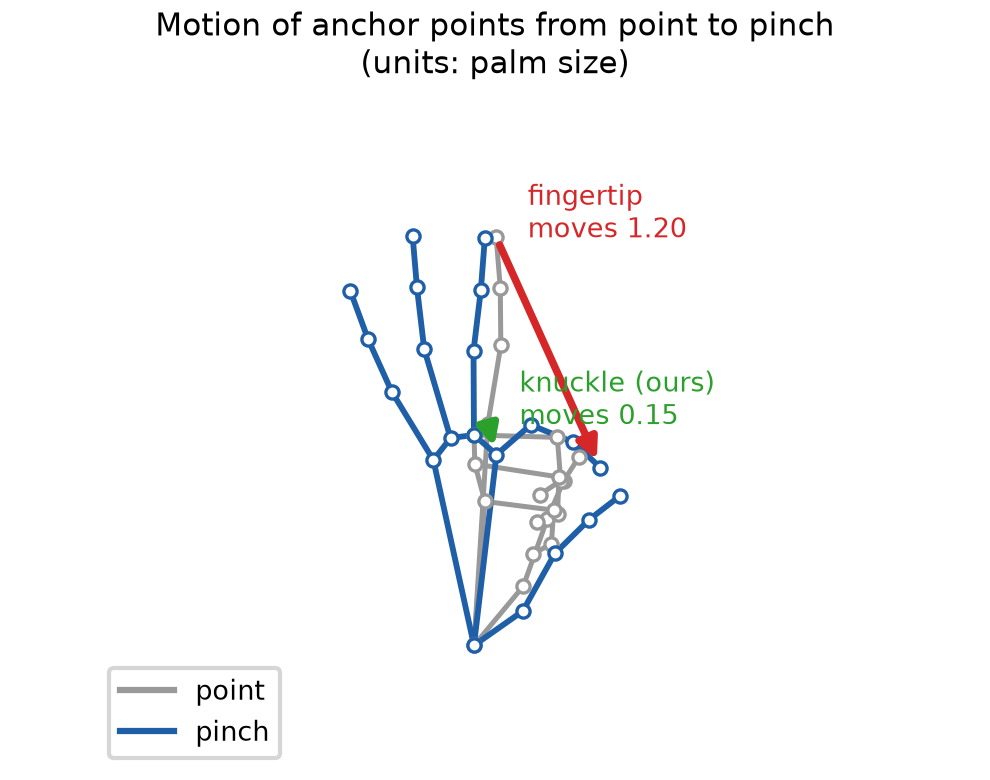
\includegraphics[width=0.85\linewidth]{figures/anchor.png}
  \caption{\textbf{Why we use the knuckle.} A typical ``point'' hand (grey) and
  ``pinch'' hand (blue) from our data, placed on the same wrist. When the user
  pinches, the fingertip moves much more than the knuckle.}
  \label{fig:anchor}
\end{figure}

\subsection{Step 6: actions and the air keyboard}
\label{sec:actions}
\Cref{tab:gestures} lists what each stable gesture does. Actions are sent to
the operating system with PyAutoGUI~\cite{pyautogui}. Holding a thumbs-up for
one second switches to keyboard mode. A QWERTY keyboard is then drawn on the
camera view, and the key under the index fingertip is highlighted. A pinch
types it. Here the pinch again moves the fingertip, by about one key, so we
add a \textbf{hover-lock}: we type the key that was highlighted in the last
``point'' frame \emph{before} the pinch.

\begin{table}[t]
  \centering\small
  \caption{Gestures and what they do.}
  \label{tab:gestures}
  \begin{tabular}{@{}lll@{}}
    \toprule
    Gesture & Mouse mode & Keyboard mode \\
    \midrule
    Open palm & pause (cursor stays) & -- \\
    Point (index up) & move cursor & highlight key \\
    Pinch thumb + index & left / double click & type key \\
    Pinch thumb + middle & right click & -- \\
    Two fingers up (V) & scroll & -- \\
    Fist & drag & -- \\
    Thumbs up, 1\,s & to keyboard mode & to mouse mode \\
    \bottomrule
  \end{tabular}
\end{table}

\subsection{Step 7: one-second personalization}
\label{sec:personal}
Every person makes gestures a little differently. Early layers of a network
learn general features, and the last layer is the most task-specific
one~\cite{yosinski2014transferable}. So for a new user we freeze the network and
re-train only its last layer (455 weights) on $K$ samples per gesture from that
user. This takes about one second on a CPU and can be done just before use.

\section{Experiments}
\label{sec:exp}

We now test the method step by step. The questions follow the four problems
of \cref{sec:intro}: does the classifier work on new people, does the filter
stop the shake, does voting stop false clicks, and does the knuckle stop the
jump?

\subsection{Dataset and setup}
\paragraph{Our dataset.} No public dataset has our 7 control gestures together
with hand points, so we recorded our own with our tool
\texttt{collect\_data.py}. Each of the three group members recorded every
gesture while moving the hand around the image, closer and farther, and a
little tilted. In total we have \textbf{15,378 labelled frames} (4,774 to 5,367
per person and 1,880 to 2,530 per gesture), each with its 21 hand points and
handedness, plus \textbf{7,692 hand-crop images} for the CNN baseline.

\paragraph{Two kinds of test.} In the \emph{random split}, 20\% of all frames
are kept for testing. The same people appear in training and testing, so this
test is easy. In \emph{leave-one-user-out}, we train on two people and test
on the third, for each person in turn. This is the honest test, because it is
exactly what happens when a new person uses the system.

\paragraph{Live sessions.} For the cursor experiments we ran the app and saved
every frame's raw hand points and predictions to a log. We recorded three
one-minute sessions: holding the hand still, moving the cursor around, and
pinching exactly 30 times. Because the raw data is saved, we can replay the
\emph{same} hand motion through every filter or voting setting and compare them
fairly.

\paragraph{Implementation.} Python with OpenCV~\cite{bradski2000opencv},
MediaPipe, PyTorch~\cite{paszke2019pytorch}, scikit-learn and
PyAutoGUI~\cite{pyautogui}. The MLP is trained with
AdamW~\cite{loshchilov2019adamw} (learning rate $10^{-3}$, cosine schedule,
label smoothing 0.05~\cite{szegedy2016rethinking}) for 60 epochs with batch
size 64. We keep the epoch with the best validation accuracy. Everything runs on
\Hardware; timings are for one frame on one CPU thread.

\subsection{Can it recognise the gestures?}
\label{sec:exp-cls}

\begin{table}[t]
\centering\small
\caption{Gesture classification on the random 20\% test split (accuracy and macro-F1 in \%, latency per sample on one CPU thread).}
\label{tab:ablation}
\resizebox{\ifdim\width>\linewidth\linewidth\else\width\fi}{!}{%
\begin{tabular}{@{}lcccc@{}}
\toprule
Method & Acc. & F1 & ms & Params \\
\midrule
Rule-based (fingers up) & 89.89 & 90.04 & 0.033 & -- \\
SVM (RBF), our features & 99.74 & 99.74 & 0.150 & -- \\
Random Forest, our features & \textbf{99.84} & \textbf{99.84} & 10.871 & -- \\
kNN ($k$=5), our features & 99.77 & 99.78 & 1.630 & -- \\
\midrule
MLP, raw coordinates & 99.67 & 99.67 & 0.222 & 17.3k \\
MLP, + mirror/translate/scale & 99.80 & 99.80 & 0.293 & 17.3k \\
MLP, + rotation & 99.80 & 99.80 & 0.317 & 17.3k \\
MLP, full features, no augm. & 99.77 & 99.78 & 0.776 & 20.5k \\
\textbf{MLP, full features + augm. (ours)} & 99.74 & 99.74 & 0.720 & 20.5k \\
\bottomrule
\end{tabular}}
\end{table}


\Cref{tab:ablation} shows the random split. The usual rule-based method gets
89.9\%. Every learned method gets between 99.7\% and 99.8\%, and our MLP takes
only 0.72\,ms per frame. On this easy test the learned methods are all about
equally good, and the confusion matrix (\cref{fig:cm}) shows almost no
mistakes. The cleaning steps and augmentation change little here, because
the test frames come from the same people as the training frames.

\begin{figure}[t]
  \centering
  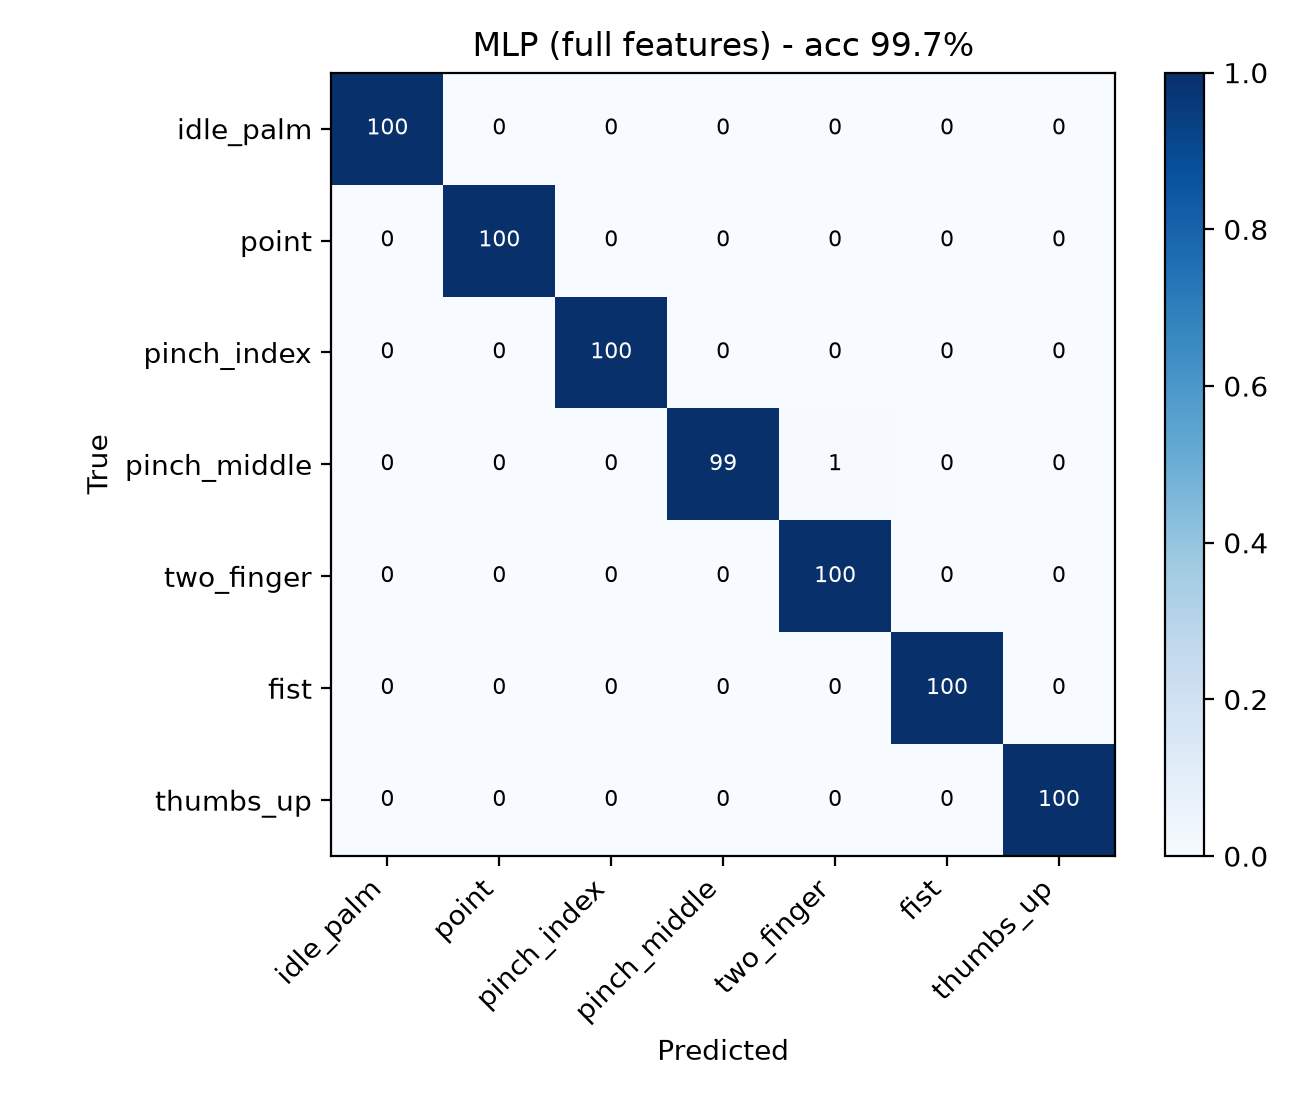
\includegraphics[width=0.9\linewidth]{figures/confusion_matrix.png}
  \caption{Confusion matrix (\%) of our MLP on the random test split.}
  \label{fig:cm}
\end{figure}

\paragraph{The real test: a new person.} \Cref{tab:loso} tells a different
story. When the person is new, the rules drop to 89.8\% and the SVM drops to
90.2\%, with only 76.5\% for Bhuvana's hand. An MLP on the raw points
without augmentation reaches 93.9\%. Our cleaned features with augmentation
reach \textbf{96.6\%} on average, and are the best for two of the three
people. So the cleaning and augmentation pay off exactly where they are needed:
on hands the model has not seen.

\begin{table}[t]
\centering\small
\caption{Leave-one-user-out accuracy (\%): trained on the other users, tested on the user in the row.}
\label{tab:loso}
\resizebox{\ifdim\width>\linewidth\linewidth\else\width\fi}{!}{%
\begin{tabular}{@{}lcccc@{}}
\toprule
Test user & Rules & SVM & MLP raw & MLP ours \\
\midrule
bhuvana & 85.15 & 76.50 & 91.24 & 94.39 \\
guna & 93.50 & 99.05 & 95.73 & 98.30 \\
raj & 90.85 & 95.04 & 94.65 & 97.23 \\
\midrule
\textbf{Mean} & \textbf{89.83} & \textbf{90.19} & \textbf{93.88} & \textbf{96.64} \\
\bottomrule
\end{tabular}}
\end{table}


\paragraph{Hand points or image pixels?} \Cref{tab:cnn} compares our MLP with
a CNN trained on the hand-crop images of the same frames. The CNN is
slightly more accurate on the random split (99.94\% vs.\ 99.74\%). However, it
is about 5.5 times slower (4.0\,ms vs.\ 0.72\,ms per frame), 12 times bigger
(242\,k vs.\ 20\,k weights), and took 455\,s to train. For a system that
must leave time for tracking and control in every frame, the small keypoint
MLP is the better choice.

\begin{table}[t]
\centering\small
\caption{Classifier on image pixels vs.\ on keypoints (same frames, random split).}
\label{tab:cnn}
\resizebox{\ifdim\width>\linewidth\linewidth\else\width\fi}{!}{%
\begin{tabular}{@{}lcccc@{}}
\toprule
Input / model & Acc. & F1 & ms & Params \\
\midrule
CNN, $64\times64$ hand image & \textbf{99.94} & \textbf{99.94} & 4.01 & 242k \\
MLP, keypoint features (ours) & 99.74 & 99.74 & 0.72 & 20.5k \\
\bottomrule
\end{tabular}}
\end{table}


\paragraph{Does personalization help?} \Cref{fig:personal} shows the accuracy
on a new user when only the last layer is re-trained with $K$ samples per
gesture. Averaged over the three of us it rises from 97.4\% ($K=0$) to
98.0\% ($K=20$). The gain is largest for the hardest user, Bhuvana: from
94.8\% to 96.7\% with 20 samples and 97.2\% with 50. For the other two, who
already started near 98--99\%, it changes little.

\begin{figure}[t]
  \centering
  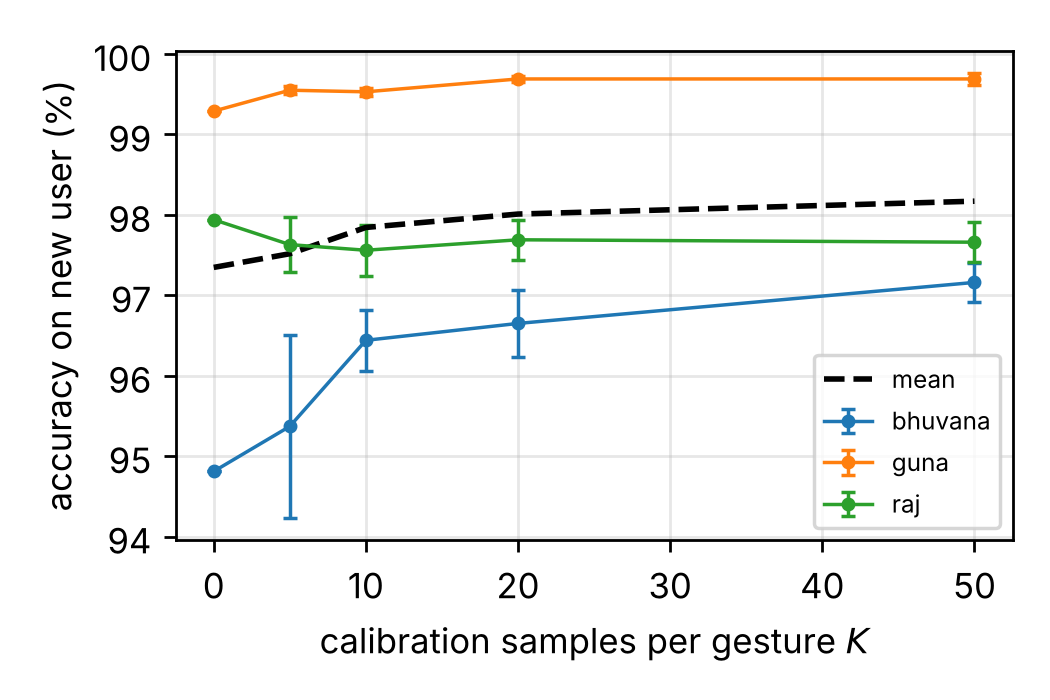
\includegraphics[width=0.85\linewidth]{figures/personalization.png}
  \caption{Accuracy on a new user against the number of calibration samples
  per gesture $K$ ($K=0$ means no calibration).}
  \label{fig:personal}
\end{figure}

\subsection{Is the cursor steady?}
\label{sec:exp-filter}
We replayed the recorded hand motion through four filters
(\cref{tab:filter,fig:trace}). \emph{Shake} is how far the cursor moves per
frame while the hand is held still. \emph{Lag} is how late the filtered cursor
is compared with the intended path.

\begin{table}[t]
\centering\small
\caption{Cursor smoothing on the same recorded hand motion (lower is better for all columns).}
\label{tab:filter}
\resizebox{\ifdim\width>\linewidth\linewidth\else\width\fi}{!}{%
\begin{tabular}{@{}lccc@{}}
\toprule
Filter & Jitter (px/frame) & Error moving (px) & Lag (ms) \\
\midrule
No filter (raw) & 4.21 & \textbf{15.19} & \textbf{0.00} \\
Moving average (5) & 3.57 & 61.52 & 64.03 \\
Kalman (const. velocity) & 3.66 & 37.64 & 32.02 \\
\textbf{One-Euro (ours)} & \textbf{2.59} & 18.82 & 10.65 \\
\bottomrule
\end{tabular}}
\end{table}


Without a filter the cursor shakes by 4.21\,px every frame. The moving
average reduces this only to 3.57\,px and adds 64\,ms of lag, so the cursor
feels like it is pulled on a rubber band. The Kalman filter is in between. The
One-Euro filter gives the \textbf{least shake (2.59\,px, 38\% less than no
filter)} with only \textbf{11\,ms} of lag. Its error while moving (18.8\,px) is
also close to the raw cursor's, while the moving average is far behind
(61.5\,px).

\begin{figure}[t]
  \centering
  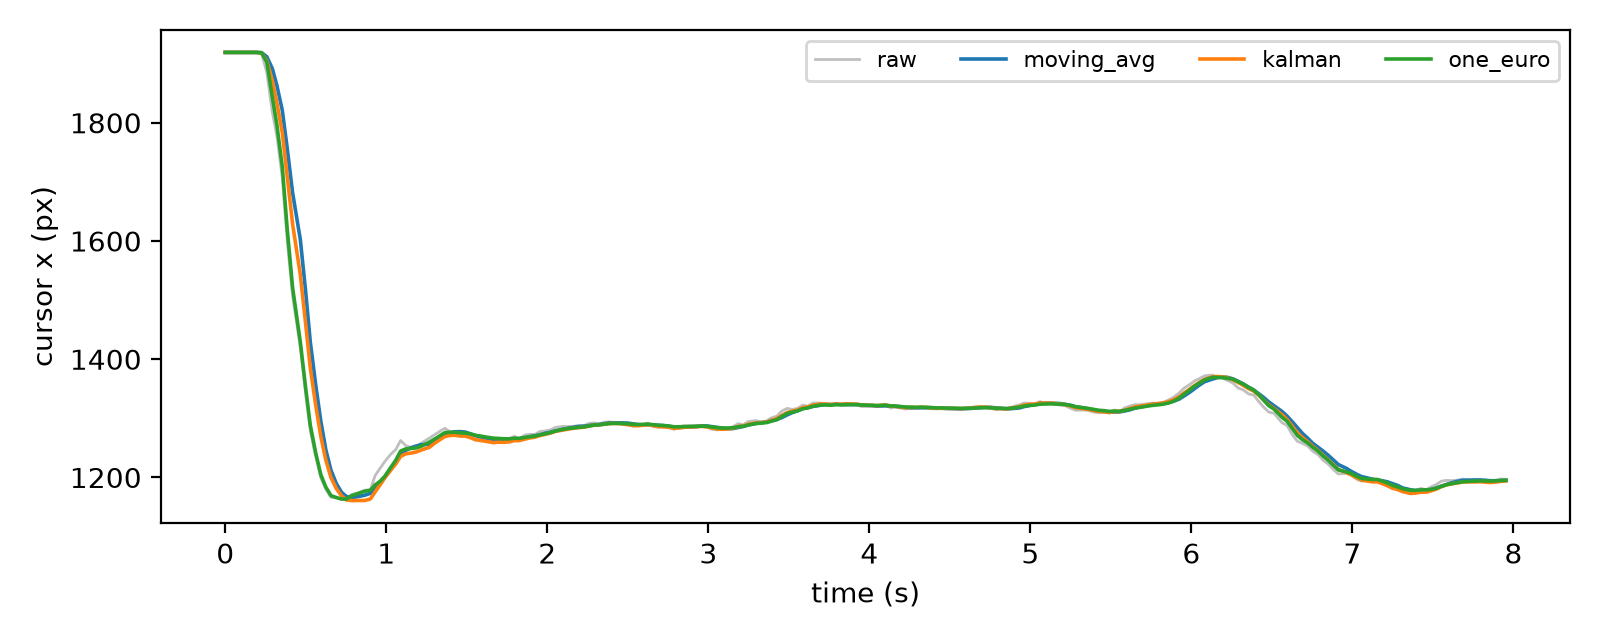
\includegraphics[width=\linewidth]{figures/filter_trace.png}
  \caption{Cursor $x$-position over time in a recorded session: raw and
  filtered.}
  \label{fig:trace}
\end{figure}

\subsection{Does voting stop false clicks?}
In the third session the user pinched exactly 30 times. We replayed the
network's frame-by-frame predictions with and without voting
(\cref{tab:voting}).

\begin{table}[t]
\centering\small
\caption{Effect of temporal voting on the same recorded predictions (the user clicked 30 times).}
\label{tab:voting}
\resizebox{\ifdim\width>\linewidth\linewidth\else\width\fi}{!}{%
\begin{tabular}{@{}lccc@{}}
\toprule
Setting & Changes/min & Short false/min & Clicks \\
\midrule
No voting (raw per-frame) & 70.0 & 31.0 & 50 \\
Voting N=3, k=2 & 24.9 & 1.2 & 32 \\
Voting N=5, k=3 (ours) & 21.2 & 0.3 & 30 \\
Voting N=7, k=5 & 18.1 & 0.0 & 28 \\
\bottomrule
\end{tabular}}
\end{table}


Without voting, the gesture changed 70 times per minute, including 31 short
false changes of one or two frames per minute, and \textbf{50 clicks} were
detected for 30 real pinches. With our setting ($N=5$, $k=3$) the short false
changes almost vanish (0.3 per minute) and \textbf{exactly 30 clicks} are
detected. A stricter setting ($N=7$, $k=5$) starts to miss real clicks (28),
so $N=5$, $k=3$ is the right balance.

\subsection{Does the knuckle stop the jump?}
For each of the 30 clicks we measured how far the cursor would move in the
four frames before the click is recognised, for three choices of anchor point
(\cref{tab:anchor}).

\begin{table}[t]
\centering\small
\caption{Cursor drift at the moment of a click for different anchor points (screen pixels, 1920$\times$1080).}
\label{tab:anchor}
\resizebox{\ifdim\width>\linewidth\linewidth\else\width\fi}{!}{%
\begin{tabular}{@{}lccc@{}}
\toprule
Anchor & Mean (px) & Median (px) & Clicks \\
\midrule
Index fingertip (usual) & 182.5 & 161.1 & 30 \\
\textbf{Index knuckle (ours)} & 53.4 & 51.5 & 30 \\
Palm centre & \textbf{52.1} & \textbf{48.9} & 30 \\
\bottomrule
\end{tabular}}
\end{table}


With the fingertip, the cursor moves \textbf{183\,px} on average during a
click, which is enough to miss most buttons. With the knuckle it moves only
\textbf{53\,px}, about 3.4 times less. The palm centre is about as stable
(52\,px), but it sits away from the pointing finger and moves when the wrist
bends, so pointing with it feels less natural. We therefore keep the knuckle.

\subsection{Is it fast enough?}
Over 7,570 logged frames the complete system ran at \textbf{32.2 frames per
second}, with 11.5\,ms of processing per frame on average (14.8\,ms in the
slowest 5\% of frames). It works in real time on an ordinary laptop CPU
(\cref{tab:system}).

\begin{table}[t]
\centering\small
\caption{System performance and user tests.}
\label{tab:system}
\resizebox{\ifdim\width>\linewidth\linewidth\else\width\fi}{!}{%
\begin{tabular}{@{}lr@{}}
\toprule
Metric & Value \\
\midrule
Frame rate (FPS) & 32.2 \\
Processing per frame, mean (ms) & 11.5 \\
Processing per frame, 95th perc. (ms) & 14.8 \\
\bottomrule
\end{tabular}}
\end{table}


\subsection{Limitations}
The system follows one hand at a time, and the hand must stay inside the
active area. Dark rooms and fast motion blur make MediaPipe lose the hand.
Typing on the air keyboard is much slower than on a real keyboard, so it is
meant for short text such as a search word. Finally, our data and tests come
from only three people.

\section{Conclusion}
\label{sec:conclusion}

We started with a simple question: can a webcam replace the mouse and the
keyboard? Existing virtual mice showed that it is possible, but also that they
are fragile, shaky and click by mistake. We went after each of these problems
and measured every fix. Cleaning the hand points and learning the gestures
with a small network raised accuracy on a new person from 89.8\% to 96.6\%.
The One-Euro filter cut the cursor shake by 38\% with only 11\,ms of delay.
Voting turned 50 detected clicks into exactly the 30 the user made, and the
knuckle anchor cut the cursor jump during a click from 183\,px to 53\,px. The
system runs at 32 frames per second on a laptop CPU, and a new user can
personalise it in about a second. In future we would like to add moving
gestures such as swipes, a relative ``lift and place'' cursor mode, and tests
with many more people.

\section*{Individual contributions}
\begin{itemize}\setlength\itemsep{1pt}
\item \textbf{Guna Sekhar Subbarao Karanam (230537):} Gesture recognition: data-collection tool, invariant feature design, Gesture MLP training with augmentation, ablation study, baselines (rules, SVM, RF, kNN, image CNN) and leave-one-user-out evaluation.
\item \textbf{VOOBA RAJKUMAR (231173):} Cursor control: stable anchor point, One-Euro / Kalman / moving-average filters, confidence + temporal voting, click / scroll / drag logic, recording and analysis of the live cursor sessions.
\item \textbf{GBHUVANA REDDY (230408):} User interface and air keyboard with hover-lock, few-shot personalization, figures, report and presentation.
\end{itemize}


{
    \small
    \bibliographystyle{ieeenat_fullname}
    \bibliography{main}
}

\clearpage
\onecolumn
\appendix
\section{Code, repository and datasets}
\label{sec:appendix}

\noindent\textbf{Our GitHub repository:} \url{\GitHubURL}

\medskip
\noindent\textbf{Datasets used.}
\begin{itemize}
\item Our own recorded dataset (15,378 labelled hand-point frames and 7,692
hand-crop images from 3 users, 7 gestures), in the repository under
\texttt{data/}.
\item Related public dataset (not used for training, listed for reference):
HaGRID~\cite{kapitanov2024hagrid}, \url{https://github.com/hukenovs/hagrid}.
\end{itemize}

\noindent\textbf{Repositories and libraries used.}
\begin{itemize}
\item MediaPipe (hand landmarks): \url{https://github.com/google-ai-edge/mediapipe}
\item OpenCV (camera and drawing): \url{https://github.com/opencv/opencv}
\item PyTorch (neural networks): \url{https://github.com/pytorch/pytorch}
\item scikit-learn (SVM, Random Forest, kNN baselines): \url{https://github.com/scikit-learn/scikit-learn}
\item PyAutoGUI (mouse and keyboard events): \url{https://github.com/asweigart/pyautogui}
\item python-pptx (slides): \url{https://github.com/scanny/python-pptx}
\item CVPR author kit (this template): \url{https://github.com/cvpr-org/author-kit}
\item One-Euro filter reference page: \url{https://gery.casiez.net/1euro/}
\end{itemize}

\noindent\textbf{How to run.} \texttt{pip install -r requirements.txt};
record data with \texttt{python collect\_data.py --user NAME}; run every
experiment with \texttt{python run\_all.py}; start the app with
\texttt{python app.py}. Details are in \texttt{README.md}.

\section{Complete source code}
\subsection*{\texttt{app.py}}
\lstinputlisting{code/app.py}
\subsection*{\texttt{collect\_data.py}}
\lstinputlisting{code/collect_data.py}
\subsection*{\texttt{config.py}}
\lstinputlisting{code/config.py}
\subsection*{\texttt{controller.py}}
\lstinputlisting{code/controller.py}
\subsection*{\texttt{features.py}}
\lstinputlisting{code/features.py}
\subsection*{\texttt{filters.py}}
\lstinputlisting{code/filters.py}
\subsection*{\texttt{hand\_tracker.py}}
\lstinputlisting{code/hand_tracker.py}
\subsection*{\texttt{make\_figures.py}}
\lstinputlisting{code/make_figures.py}
\subsection*{\texttt{make\_report.py}}
\lstinputlisting{code/make_report.py}
\subsection*{\texttt{make\_slides.py}}
\lstinputlisting{code/make_slides.py}
\subsection*{\texttt{make\_slides\_full.py}}
\lstinputlisting{code/make_slides_full.py}
\subsection*{\texttt{model.py}}
\lstinputlisting{code/model.py}
\subsection*{\texttt{personalize.py}}
\lstinputlisting{code/personalize.py}
\subsection*{\texttt{rules.py}}
\lstinputlisting{code/rules.py}
\subsection*{\texttt{run\_all.py}}
\lstinputlisting{code/run_all.py}
\subsection*{\texttt{train.py}}
\lstinputlisting{code/train.py}
\subsection*{\texttt{train\_cnn.py}}
\lstinputlisting{code/train_cnn.py}
\subsection*{\texttt{virtual\_keyboard.py}}
\lstinputlisting{code/virtual_keyboard.py}
\subsection*{\texttt{voting.py}}
\lstinputlisting{code/voting.py}
\subsection*{\texttt{experiments/analyze\_logs.py}}
\lstinputlisting{code/experiments__analyze_logs.py}
\subsection*{\texttt{experiments/click\_test.py}}
\lstinputlisting{code/experiments__click_test.py}
\subsection*{\texttt{experiments/typing\_test.py}}
\lstinputlisting{code/experiments__typing_test.py}



\end{document}
